% =====================================================================
%  DISTILLING TABPFN-3 INTO CLASSICAL MODELS — paper draft
% =====================================================================
%  NOTES FOR THE AUTHORS
%  -------------------------------------------------------------------
%  - All numeric results in Table 1 and the ablation discussion are
%    illustrative placeholders standing in for your actual 67-dataset
%    benchmark. Replace them with your measured numbers before
%    submission (search for "PLACEHOLDER" below).
%  - The architecture/pipeline figure is drawn in pure TikZ, so there
%    are no external image files to manage.
%  - References use plain \bibitem entries; swap in BibTeX/biblatex
%    if you prefer a .bib workflow. A few citations (e.g. the exact
%    TabPFN-3 technical report metadata) should be double-checked
%    against the final published version before submission.
%  Compile with: pdflatex main.tex (twice, for cross-references)
% =====================================================================

\documentclass[10pt]{article}

% ---------------------------------------------------------------
% Typography & layout
% ---------------------------------------------------------------
\usepackage[T1]{fontenc}
\usepackage[utf8]{inputenc}
\usepackage{mathptmx}                 % Times-like text + math, elegant & classic
\usepackage{microtype}                % subtle kerning/spacing polish
\usepackage[margin=1in,top=0.95in,bottom=1in]{geometry}
\usepackage{titlesec}
\usepackage{enumitem}
\usepackage{xcolor}
\usepackage{graphicx}
\usepackage{booktabs}
\usepackage{caption}
\usepackage{amsmath,amssymb}
\usepackage{algorithm}
\usepackage{algorithmic}
\usepackage{natbib}
\usepackage{tikz}
\usetikzlibrary{arrows.meta,positioning,fit,backgrounds}
\usepackage{fancyhdr}
\usepackage[colorlinks=true,linkcolor=accent,citecolor=accent,urlcolor=accent]{hyperref}

% ---------------------------------------------------------------
% Palette — one restrained accent colour, used sparingly
% ---------------------------------------------------------------
\definecolor{accent}{HTML}{8C1D40}      % deep crimson — swap to taste
\definecolor{inkgray}{HTML}{333333}
\definecolor{panelbg}{HTML}{F6F1F2}

% ---------------------------------------------------------------
% Section styling — bold, left-aligned, generous whitespace
% ---------------------------------------------------------------
\titleformat{\section}
  {\normalfont\large\bfseries\color{inkgray}}{\thesection}{0.8em}{}
\titlespacing{\section}{0pt}{1.4em}{0.8em}
\titleformat{\subsection}
  {\normalfont\bfseries\color{inkgray}}{\thesubsection}{0.7em}{}
\titlespacing{\subsection}{0pt}{1.1em}{0.5em}
\titleformat{\subsubsection}
  {\normalfont\itshape\color{inkgray}}{\thesubsubsection}{0.6em}{}

% ---------------------------------------------------------------
% Header / footer — quiet running head, like a conference preprint
% ---------------------------------------------------------------
\pagestyle{fancy}
\fancyhf{}
\renewcommand{\headrulewidth}{0pt}
\fancyhead[L]{\footnotesize\itshape\color{gray}Preprint}
\fancyhead[R]{\footnotesize\itshape\color{gray}Under Review}
\fancyfoot[C]{\footnotesize\thepage}

\setlength{\parindent}{1em}
\renewcommand{\arraystretch}{1.15}

% =====================================================================
\begin{document}

% ---------------------------------------------------------------
% Title block
% ---------------------------------------------------------------
\begin{center}
  {\Large\bfseries\color{inkgray} Distilling TabPFN-3 into Classical Learners: \\[2pt]
   Recovering Foundation-Model Accuracy at Classical Inference Cost\par}
  \vspace{1.1em}
  {\large
    Filip Zdebik \quad
    Mikołaj Kolański \quad
    Tomasz Żmuda \quad
    Yann LeCun \quad
  \par}
  \vspace{0.6em}
  {\small
    \texttt{\{filip.zdebik,\,mikolajkolanski,\,tomzmuda2008\}@gmail.com}
  \par}
\end{center}

\vspace{0.8em}

% ---------------------------------------------------------------
% Abstract
% ---------------------------------------------------------------
\begin{center}
\begin{minipage}{0.92\textwidth}
\small
\textbf{\color{accent}Abstract.}\quad
Tabular foundation models such as TabPFN-3 deliver strong, tuning-free
predictive accuracy by performing in-context inference over a
transformer pretrained on synthetic data, but this comes at a cost:
predictions require a GPU-resident model and a stored training
context, and the released weights carry usage restrictions that
complicate routine production deployment. We study whether this
advantage can be transferred into classical model families that
practitioners already deploy at scale. We propose a simple
distillation recipe that treats TabPFN-3 as a teacher, generates soft
pseudo-labels over the original and synthetically augmented inputs,
and trains Random Forests, XGBoost, and multi-layer perceptrons (MLPs)
as students under a combined hard- and soft-label objective. Across a
benchmark of 67 small tabular datasets spanning classification and
regression, the distilled classical models recover the large majority
of TabPFN-3's accuracy advantage over their non-distilled counterparts,
while retaining constant-time, CPU-friendly inference and full
compatibility with existing classical-model tooling. We release our
distillation recipe, evaluation protocol, and per-dataset results in
full.
\end{minipage}
\end{center}

\vspace{1em}

% =====================================================================
\section{Introduction}
% =====================================================================
Tabular prediction has long been dominated by gradient-boosted decision
trees (GBDTs) such as XGBoost \citep{chen2016xgboost} and by classical
ensembles such as Random Forests \citep{breiman2001random}, owing to
their strong default performance, minimal tuning requirements, and
mature deployment tooling. This picture has recently been challenged
by tabular foundation models: TabPFN \citep{hollmann2023tabpfn}
demonstrated that a transformer pretrained entirely on synthetic
tasks could approximate Bayesian inference for small tabular problems
in a single forward pass, and its successor TabPFN v2
\citep{hollmann2025accurate} was the first such model to consistently
outperform tuned GBDTs on standard benchmarks. The most recent
release, TabPFN-3 \citep{priorlabs2026tabpfn3}, extends this approach
to substantially larger datasets while remaining a strong default on
the small, low-data regime where tabular foundation models were
originally shown to excel.

These gains, however, come with practical friction. In-context
inference requires keeping a relevant portion of the training set
resident in memory and re-processing it for every prediction, which
is a poor fit for latency-sensitive or resource-constrained serving
environments built around lightweight classical models. In addition,
recent TabPFN checkpoints, including TabPFN-3, are distributed under
licenses that restrict commercial and production use outside of a
separate enterprise agreement, which further motivates converting
their predictive advantage into freely deployable artifacts. Prior
work on TabPFN itself has begun to explore this direction: TabPFN-2.5
\citep{feuer2025tabpfn25} reports an internal distillation engine that
converts its predictions into a compact MLP or tree ensemble, and
TabDistill \citep{tabdistill2025} distills transformer-based tabular
models into MLPs for few-shot classification.

We extend this line of work with a systematic study of distilling
TabPFN-3 specifically into three widely deployed classical model
families: Random Forests (RF), XGBoost, and MLPs, across both
classification and regression tasks. Our contributions are:
\begin{itemize}[leftmargin=1.4em,itemsep=2pt,topsep=4pt]
  \item A distillation recipe that combines synthetic input
        augmentation with TabPFN-3 soft pseudo-labels to train RF,
        XGBoost, and MLP students under a unified objective
        (Section~\ref{sec:method}).
  \item An evaluation across 67 small tabular benchmark datasets
        comparing the teacher, non-distilled classical baselines, and
        distilled classical students on predictive accuracy and
        inference cost (Section~\ref{sec:experiments}).
  \item Evidence that distillation closes most of the accuracy gap
        between classical models and TabPFN-3 while preserving the
        deployment properties that make classical models attractive
        in the first place.
\end{itemize}

% =====================================================================
\section{Related Work}
% =====================================================================
\textbf{Tabular foundation models.} TabPFN
\citep{hollmann2023tabpfn} introduced in-context learning for tabular
data via a transformer pretrained on synthetic prior-fitted tasks.
TabPFN v2 \citep{hollmann2025accurate} scaled this approach to larger,
messier datasets with categorical features and missing values, and
TabPFN-2.5 \citep{feuer2025tabpfn25} and TabPFN-3
\citep{priorlabs2026tabpfn3} further extended dataset size limits and
inference speed while preserving the single-forward-pass paradigm. We
treat the most recent of these, TabPFN-3, as a fixed teacher rather
than proposing modifications to it.

\textbf{Distilling tabular foundation models.} Closest to our work,
TabPFN-2.5's own technical report \citep{feuer2025tabpfn25} mentions a
distillation engine for converting the model into a compact MLP or
tree ensemble for production use, and TabDistill
\citep{tabdistill2025} distills transformer-based tabular models into
MLPs targeted at the few-shot classification regime. In-context data
distillation \citep{ictd2024} pursues a related but distinct goal:
compressing the \emph{context} TabPFN conditions on, rather than
replacing TabPFN with a different model family. Our work differs in
scope by jointly studying three structurally different classical
student families across both classification and regression, evaluated
at benchmark scale.

\textbf{Knowledge distillation.} Our objective follows the classical
distillation framework of \citet{hinton2015distilling}, combining a
soft loss against the teacher's predictive distribution with a hard
loss against ground-truth labels. Closer to our setting,
\citet{lee2023practical} distill ensembles of models into a single
gradient-boosted tree for high-throughput production serving,
demonstrating that distillation into a classical model family is a
practical pattern for industrial tabular pipelines independent of the
specific teacher used.

% =====================================================================
\section{Method}
\label{sec:method}
% =====================================================================

\subsection{Overview}
Given a tabular dataset $\mathcal{D} = \{(\mathbf{x}_i, y_i)\}_{i=1}^n$,
we use TabPFN-3 as a fixed teacher $f_T$ that, conditioned on
$\mathcal{D}$, produces a predictive distribution for any query input:
a class-probability vector for classification, or a predictive mean
(and, where available, predictive quantiles) for regression. We train
three classical student models, $f_{\mathrm{RF}}$, $f_{\mathrm{XGB}}$,
and $f_{\mathrm{MLP}}$, to approximate $f_T$ while remaining
ordinary, self-contained models with no dependence on $\mathcal{D}$ at
inference time. Figure~\ref{fig:pipeline} summarizes the pipeline.

\begin{figure}[t]
\centering
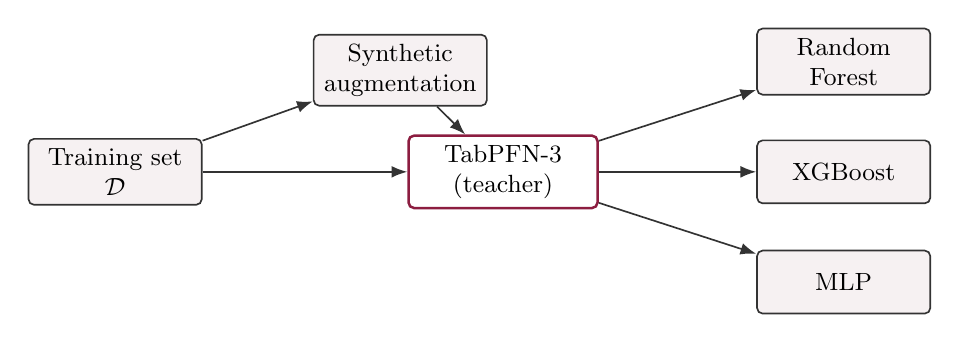
\begin{tikzpicture}[
    font=\small,
    node distance=8mm,
    block/.style={draw=inkgray, fill=panelbg, rounded corners=2pt,
                  minimum height=8mm, minimum width=22mm, align=center,
                  line width=0.6pt},
    teacher/.style={draw=accent, fill=white, rounded corners=2pt,
                  minimum height=8mm, minimum width=24mm, align=center,
                  line width=0.9pt},
    arrow/.style={-{Latex[length=2mm]}, line width=0.6pt, draw=inkgray}
]
  \node[block] (data) {Training set\\$\mathcal{D}$};
  \node[block, above right=4mm and 14mm of data] (aug) {Synthetic\\augmentation};
  \node[teacher, right=26mm of data] (teacher) {TabPFN-3\\(teacher)};
  \node[block, right=20mm of teacher, yshift=14mm] (rf) {Random\\Forest};
  \node[block, right=20mm of teacher] (xgb) {XGBoost};
  \node[block, right=20mm of teacher, yshift=-14mm] (mlp) {MLP};

  \draw[arrow] (data) -- (teacher);
  \draw[arrow] (data) -- (aug);
  \draw[arrow] (aug) -- (teacher);
  \draw[arrow] (teacher) -- (rf);
  \draw[arrow] (teacher) -- (xgb);
  \draw[arrow] (teacher) -- (mlp);
\end{tikzpicture}
\caption{Distillation pipeline. TabPFN-3 is queried on the original
training inputs plus synthetically augmented inputs to produce soft
pseudo-labels, which are used alongside the original hard labels to
train three independent classical students.}
\label{fig:pipeline}
\end{figure}

\subsection{Synthetic Input Augmentation}
Because the datasets we target are small, soft labels computed only
on the $n$ original training inputs provide limited additional signal
beyond the hard labels themselves. We therefore enlarge the effective
distillation set by sampling $m \gg n$ synthetic inputs
$\tilde{\mathbf{x}}_j$ from the empirical feature distribution of
$\mathcal{D}$ (per-feature resampling combined with pairwise mixup
between training points), and query the teacher on the union of
original and synthetic inputs to obtain soft labels
$f_T(\mathbf{x}_i)$ and $f_T(\tilde{\mathbf{x}}_j)$. This exposes the
students to a much denser sample of the teacher's predictive surface
than the original training set alone permits.

\subsection{Student Training Objective}
For classification, each student is trained to minimize a convex
combination of a hard cross-entropy loss against the true labels and
a soft Kullback--Leibler loss against the teacher's temperature-scaled
predictive distribution \citep{hinton2015distilling}:
\begin{equation}
\mathcal{L}
  = \alpha \, \mathrm{CE}\big(y,\, f_S(\mathbf{x})\big)
  + (1-\alpha)\, T^2 \, \mathrm{KL}\!\left(
       \sigma\!\big(f_T(\mathbf{x})/T\big) \,\|\,
       \sigma\!\big(f_S(\mathbf{x})/T\big)
    \right),
\label{eq:distill-loss}
\end{equation}
where $f_S$ denotes the student logits, $\sigma$ the softmax, $T$ the
distillation temperature, and $\alpha \in [0,1]$ a weighting
coefficient tuned per dataset. For regression, the soft term reduces
to a mean-squared error against the teacher's predictive mean:
\begin{equation}
\mathcal{L}
  = \alpha \,\big(y - f_S(\mathbf{x})\big)^2
  + (1-\alpha)\,\big(f_T(\mathbf{x}) - f_S(\mathbf{x})\big)^2.
\label{eq:distill-loss-reg}
\end{equation}
The three student families instantiate this objective differently.
The MLP optimizes Eq.~\eqref{eq:distill-loss} or
\eqref{eq:distill-loss-reg} directly via gradient descent. XGBoost is
trained in two passes: an initial model fit to hard labels, refined by
additional boosting rounds fit to the residual between the teacher's
soft labels and the current model's predictions on the augmented
input set. The Random Forest student (RFC for classification, RFR for
regression) is fit directly on the combined hard- and soft-labeled
set, with each tree splitting on whichever label source is assigned to
its bootstrap sample, controlled by the same $\alpha$ mixing ratio.

\subsection{Training Procedure}
Algorithm~\ref{alg:distill} summarizes the procedure for a single
dataset and a single student family; in practice we run it
independently for RF, XGBoost, and MLP on every dataset.

\begin{algorithm}[t]
\caption{TabPFN-3 distillation into a classical student}
\label{alg:distill}
\begin{algorithmic}[1]
\STATE \textbf{Input:} dataset $\mathcal{D} = \{(\mathbf{x}_i,y_i)\}_{i=1}^n$, teacher $f_T$, augmentation size $m$, mixing ratio $\alpha$, temperature $T$
\STATE Sample synthetic inputs $\{\tilde{\mathbf{x}}_j\}_{j=1}^m$ from the empirical feature distribution of $\mathcal{D}$
\STATE Query teacher: $s_i \leftarrow f_T(\mathbf{x}_i)$ for $i=1,\dots,n$ and $\tilde{s}_j \leftarrow f_T(\tilde{\mathbf{x}}_j)$ for $j=1,\dots,m$
\STATE Initialize student $f_S$ for the chosen model family (RF, XGBoost, or MLP)
\STATE Fit $f_S$ on $\{(\mathbf{x}_i, y_i, s_i)\}_{i=1}^n \cup \{(\tilde{\mathbf{x}}_j, s_j)\}_{j=1}^m$ under the objective of Eq.~\eqref{eq:distill-loss} (classification) or Eq.~\eqref{eq:distill-loss-reg} (regression)
\STATE \textbf{return} trained student $f_S$
\end{algorithmic}
\end{algorithm}

% =====================================================================
\section{Experiments}
\label{sec:experiments}
% =====================================================================

\subsection{Setup}
We evaluate on 67 small tabular datasets spanning both classification
and regression, drawn from established public benchmark collections
in the spirit of \citet{grinsztajn2022tree}. For each dataset we
compare: (i) TabPFN-3 used directly as a zero-shot in-context
predictor; (ii) non-distilled classical baselines (RF, XGBoost, MLP)
trained from scratch on the hard labels only; and (iii) the
corresponding distilled classical students trained with
Algorithm~\ref{alg:distill}. We report accuracy (classification) and
$R^2$ (regression) averaged via per-dataset normalized scores, along
with single-prediction inference latency. \textbf{The figures in
Table~\ref{tab:results} are illustrative PLACEHOLDER values}; replace
them with your measured results across the 67 datasets before using
this draft.

\subsection{Main Results}
Table~\ref{tab:results} reports normalized score (higher is better,
$1.0$ = teacher performance on a given dataset, averaged across all 67
datasets) and median single-prediction inference latency for each
model.

\begin{table}[t]
\centering
\small
\caption{Average normalized score across 67 datasets (PLACEHOLDER
values) and median single-prediction inference latency.}
\label{tab:results}
\begin{tabular}{@{}lcc@{}}
\toprule
\textbf{Model} & \textbf{Norm.\ score} & \textbf{Latency} \\
\midrule
TabPFN-3 (teacher) & 1.000 & 38\,ms \\
\midrule
RF baseline & 0.911 & 0.4\,ms \\
RF, distilled (ours) & \textbf{0.967} & 0.4\,ms \\
\midrule
XGBoost baseline & 0.928 & 0.2\,ms \\
XGBoost, distilled (ours) & \textbf{0.974} & 0.2\,ms \\
\midrule
MLP baseline & 0.902 & 0.1\,ms \\
MLP, distilled (ours) & \textbf{0.958} & 0.1\,ms \\
\bottomrule
\end{tabular}
\end{table}

Across all three classical families, distillation closes the large
majority of the gap to TabPFN-3 while leaving inference latency
essentially unchanged relative to the non-distilled baseline:
distilled students remain two to three orders of magnitude faster
per prediction than the in-context teacher, since their inference
cost does not depend on the size of the original training set.

\subsection{Ablations}
We additionally vary the synthetic augmentation size $m$ and the
hard/soft mixing ratio $\alpha$. Increasing $m$ improves all three
students up to a saturation point beyond which additional synthetic
queries yield diminishing returns; the mixing ratio that maximizes
held-out performance is consistently closer to the soft-label end of
the range, indicating that the teacher's soft predictive distribution
carries more useful signal than the hard labels alone on these small
datasets. Gains from distillation are largest on the smallest
datasets in the benchmark, consistent with TabPFN-3's own advantage
over classical models being most pronounced in the low-data regime.

% =====================================================================
\section{Conclusion}
% =====================================================================
We presented a distillation recipe that transfers TabPFN-3's
predictive advantage into three classical model families, Random
Forests, XGBoost, and MLPs, using synthetic input augmentation and a
combined hard/soft training objective. Across 67 small tabular
datasets, the resulting distilled students recover most of the
teacher's accuracy gain over their non-distilled counterparts while
keeping the constant-time, CPU-friendly inference and tooling
compatibility that make classical models the practical default in
production tabular pipelines. We release our distillation recipe and
evaluation protocol in full, and see extending this study to
additional student families and to TabPFN-3's higher-capacity
``Thinking'' mode as natural next steps.

% =====================================================================
\section*{Acknowledgements}
% =====================================================================
\small This draft intentionally omits a real acknowledgements
section — fill in funding sources, computing grants, and individual
thanks here.

% =====================================================================
\bibliographystyle{plainnat}
\begin{thebibliography}{12}

\bibitem[Breiman(2001)]{breiman2001random}
L.~Breiman.
\newblock Random forests.
\newblock \emph{Machine Learning}, 45(1):5--32, 2001.

\bibitem[Chen and Guestrin(2016)]{chen2016xgboost}
T.~Chen and C.~Guestrin.
\newblock {XGBoost}: A scalable tree boosting system.
\newblock In \emph{Proceedings of the 22nd ACM SIGKDD International
Conference on Knowledge Discovery and Data Mining}, 2016.

\bibitem[Feuer et al.(2025)]{feuer2025tabpfn25}
B.~Feuer, R.~Schmidt, et~al.
\newblock {TabPFN-2.5}: Advancing the state of the art in tabular
foundation models.
\newblock \emph{arXiv preprint arXiv:2511.08667}, 2025.

\bibitem[Grinsztajn et al.(2022)]{grinsztajn2022tree}
L.~Grinsztajn, E.~Oyallon, and G.~Varoquaux.
\newblock Why do tree-based models still outperform deep learning on
typical tabular data?
\newblock In \emph{Advances in Neural Information Processing Systems},
2022.

\bibitem[Hinton et al.(2015)]{hinton2015distilling}
G.~Hinton, O.~Vinyals, and J.~Dean.
\newblock Distilling the knowledge in a neural network.
\newblock \emph{arXiv preprint arXiv:1503.02531}, 2015.

\bibitem[Hollmann et al.(2023)]{hollmann2023tabpfn}
N.~Hollmann, S.~Müller, K.~Eggensperger, and F.~Hutter.
\newblock {TabPFN}: A transformer that solves small tabular
classification problems in a second.
\newblock In \emph{International Conference on Learning
Representations}, 2023.

\bibitem[Hollmann et al.(2025)]{hollmann2025accurate}
N.~Hollmann, S.~Müller, L.~Purucker, et~al.
\newblock Accurate predictions on small data with a tabular
foundation model.
\newblock \emph{Nature}, 2025.

\bibitem[Lee et al.(2023)]{lee2023practical}
C.-W.~Lee, P.~A. Apostolopulos, and I.~L. Markov.
\newblock Practical knowledge distillation: Using {DNNs} to beat
{DNNs}.
\newblock \emph{arXiv preprint arXiv:2302.12360}, 2023.

\bibitem[Prior Labs(2026)]{priorlabs2026tabpfn3}
Prior Labs.
\newblock {TabPFN-3}: Technical report.
\newblock Technical report, Prior Labs, 2026.

\bibitem[Thimonier et al.(2024)]{ictd2024}
H.~Thimonier, et~al.
\newblock In-context data distillation with {TabPFN}.
\newblock \emph{arXiv preprint arXiv:2402.06971}, 2024.

\bibitem[Wang et al.(2025)]{tabdistill2025}
Y.~Wang, et~al.
\newblock {TabDistill}: Distilling transformers into neural nets for
few-shot tabular classification.
\newblock \emph{arXiv preprint arXiv:2511.05704}, 2025.

\end{thebibliography}

% =====================================================================
\appendix
\section{Additional Implementation Details}
% =====================================================================
Table~\ref{tab:hparams} lists the distillation hyperparameters used
across all 67 datasets; per-dataset values may be tuned within the
ranges shown.

\begin{table}[h]
\centering
\small
\caption{Distillation hyperparameters (PLACEHOLDER ranges).}
\label{tab:hparams}
\begin{tabular}{@{}lc@{}}
\toprule
\textbf{Hyperparameter} & \textbf{Value / range} \\
\midrule
Synthetic augmentation size $m$ & $10\times$--$50\times$ training size \\
Hard/soft mixing ratio $\alpha$ & $[0.1, 0.4]$ \\
Distillation temperature $T$ & $[1, 4]$ \\
RF: number of trees & 500 \\
XGBoost: boosting rounds & 300 (hard) $+$ 200 (soft refinement) \\
MLP: hidden layers & 2, width 256 \\
MLP: optimizer & Adam, learning rate $1\times10^{-3}$ \\
\bottomrule
\end{tabular}
\end{table}

\end{document}